\begin{frame}\begin{center}
		\LARGE\textit{Incarnations of the Roy Model}
\end{center}\end{frame}
%-------------------------------------------------------------------------------
%-------------------------------------------------------------------------------
\begin{frame}
	\textbf{Original Roy model}

	\begin{align*}
	\text{Potential Outcomes} &\qquad \text{Cost} \\
	W_1 = \pi_1 S_1      &\qquad C = 0 \\
	W_2 = \pi_2 S_2       &\qquad \\
	& \\
	\text{Observed Outcomes } &\qquad \text{Choice} \\
	W = D W_1 + (1 - D)W_2 &\qquad S = W_1 - W_2 \\
	&\qquad D = \mathrm{I}[S > 0] \\
	\end{align*}
\end{frame}
%-------------------------------------------------------------------------------
%-------------------------------------------------------------------------------
\begin{frame}
	\begin{figure}[htp]\centering
		\caption{Occupational sorting in the original Roy model}
		\scalebox{0.35}{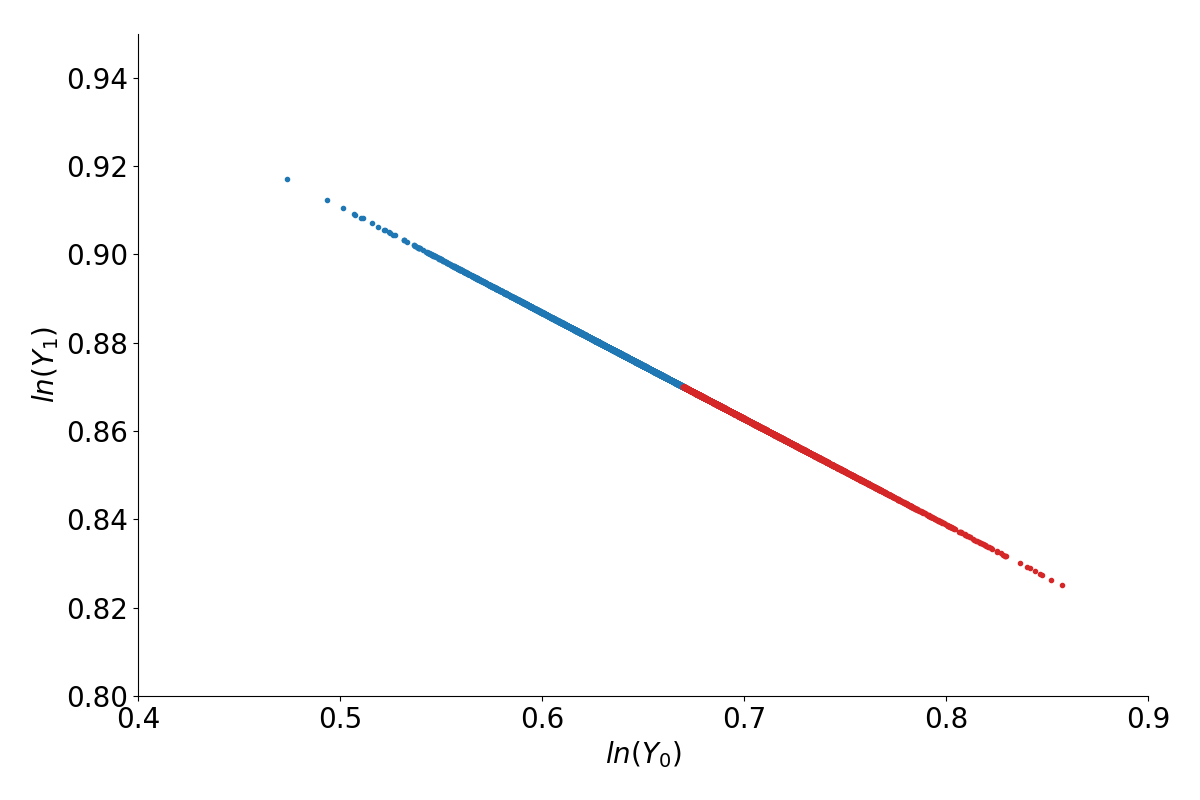
\includegraphics{fig-occupational-choices-original}}
	\end{figure}
\end{frame}
%-------------------------------------------------------------------------------
%-------------------------------------------------------------------------------
\begin{frame}
	\textbf{Extended Roy model}
	\begin{align*}
	\text{Potential Outcomes} &\qquad \text{Cost} \\
	Y_1 = \mu_1(X) + U_1      &\qquad C = \mu_D(Z) \\
	Y_0 = \mu_0(X) + U_0      &\qquad \\
	& \\
	\text{Observed Outcomes } &\qquad \text{Choice} \\
	Y = D Y_1 + (1 - D)Y_0 &\qquad S = Y_1 - Y_0 - C \\
	&\qquad D = \mathrm{I}[S > 0] \\
	\end{align*}
\end{frame}
%-------------------------------------------------------------------------------
%-------------------------------------------------------------------------------
\begin{frame}
	\begin{figure}[htp]\centering
		\caption{Occupational sorting in the extended Roy model}
		\scalebox{0.35}{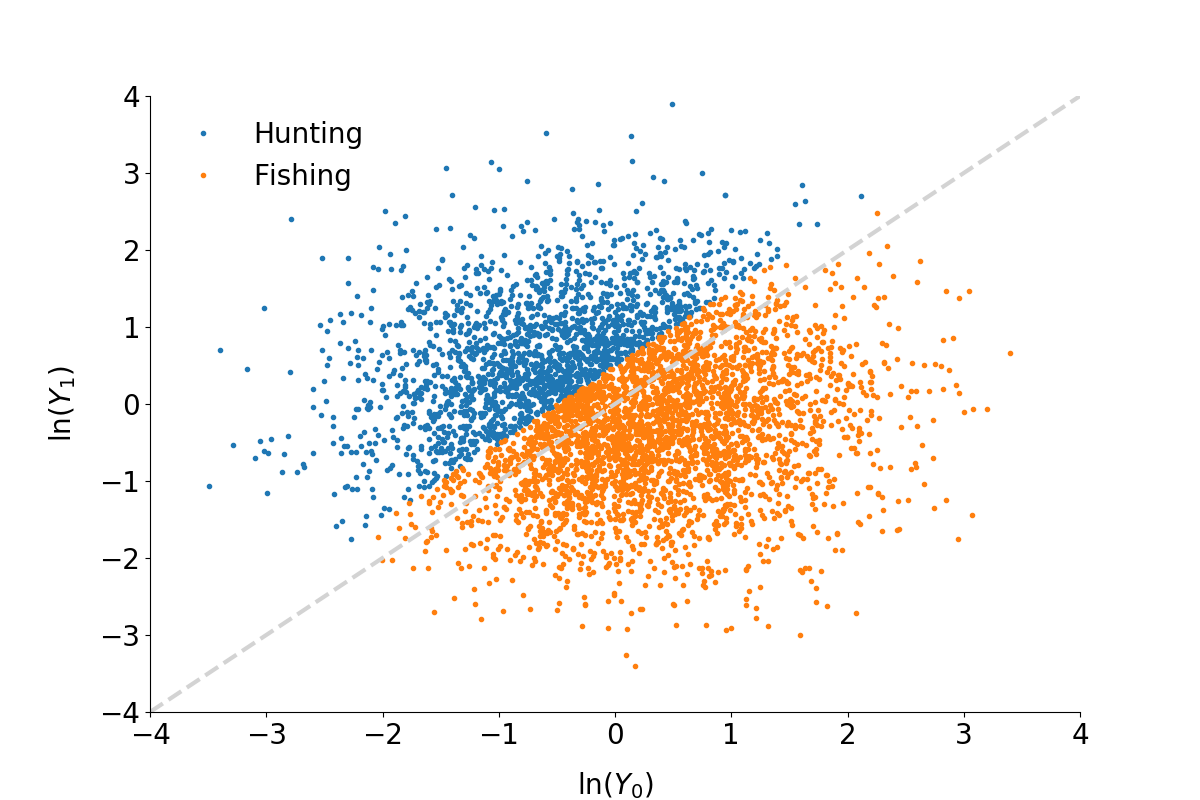
\includegraphics{fig-occupational-choices-extended}}
	\end{figure}
\end{frame}
%-------------------------------------------------------------------------------
%-------------------------------------------------------------------------------
\begin{frame}
	\textbf{Generalized Roy model}
	\begin{align*}\begin{array}{l@{\qquad}l}
			\text{Potential Outcomes} &\text{Observed Outcome}\\
			Y_1 = \mu_1(X) + U_1      &  Y = D Y_1 + (1 - D)Y_0 \\
			Y_0 = \mu_0(X) + U_0      &\\
			& \\
			\text{Choice} & \\
			D = \mathrm{I}[\mu_D(X, Z) - V > 0] & \\
		\end{array}
	\end{align*}
\end{frame}
%-------------------------------------------------------------------------------
%-------------------------------------------------------------------------------
\begin{frame}
	\begin{figure}[htp]\centering
		\caption{Occupational sorting in the generalized Roy model}
		\scalebox{0.35}{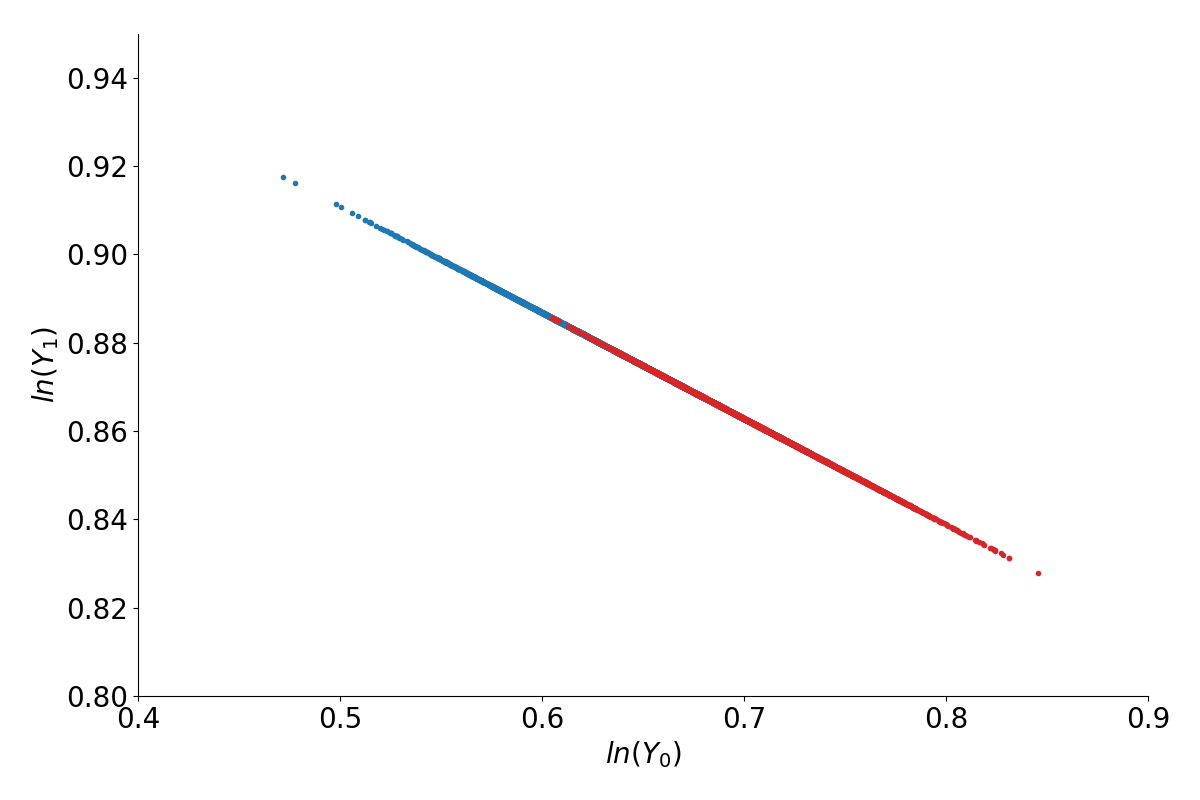
\includegraphics{fig-occupational-choices-generalized}}
	\end{figure}
\end{frame}
